%! app: regular-languages
%! outcome: Formal definition of automata, Informal definition of automata, Nondeterminism


\begin{center}
\begin{tabular}{|ll|}
\hline
\multicolumn{2}{|l|}{{\bf Nondeterministic finite automaton} $M = (Q, \Sigma, \delta, q_0, F)$} \\
Finite set of states $Q$  & Can  be labelled by any collection  of distinct names. Default: $q0, q1, \ldots$  \\
Alphabet $\Sigma$ &  Each input to the automaton is a string over  $\Sigma$. \\
Arrow labels $\Sigma_\varepsilon$ &  $\Sigma_\varepsilon = \Sigma \cup \{ \varepsilon\}$. \\
&  Arrows 
in the state diagram are labelled either by symbols from $\Sigma$ or by $\varepsilon$ \\
Transition function $\delta$  & $\delta: Q \times \Sigma_{\varepsilon} \to \mathcal{P}(Q)$
gives the {\bf set of possible next states} for a transition \\
&  from the current state upon reading a symbol or spontaneously moving.\\
Start state $q_0$ & Element of $Q$.  Each computation of the machine starts at the  start  state.\\
Accept (final) states $F$ & $F \subseteq  Q$.\\
$M$ accepts the input string & if and only if {\bf there is} a computation of $M$ on the input string\\
&  that 
processes the whole string and ends in an
accept state.\\
\hline
{\it Page 53}& \\
\hline
\end{tabular}
\end{center}

The formal definition of the NFA over $\{0,1\}$ given by this state diagram is: 

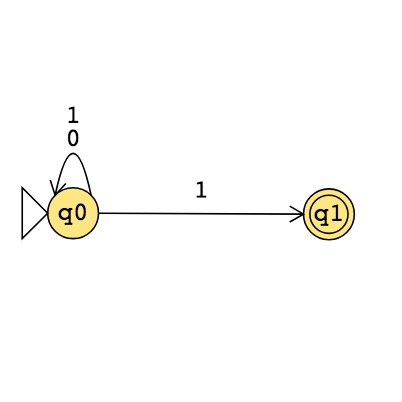
\includegraphics[width=2in]{../../resources/machines/Lect4NFA1.png}

The language over $\{0,1\}$ recognized by this NFA is:

\vspace{70pt}

Change the transition function to get a different NFA which accepts
the empty string.


\newpage

The state diagram of an NFA over $\{a,b\}$ is below.  The formal definition of this NFA is:

\vspace{-30pt}

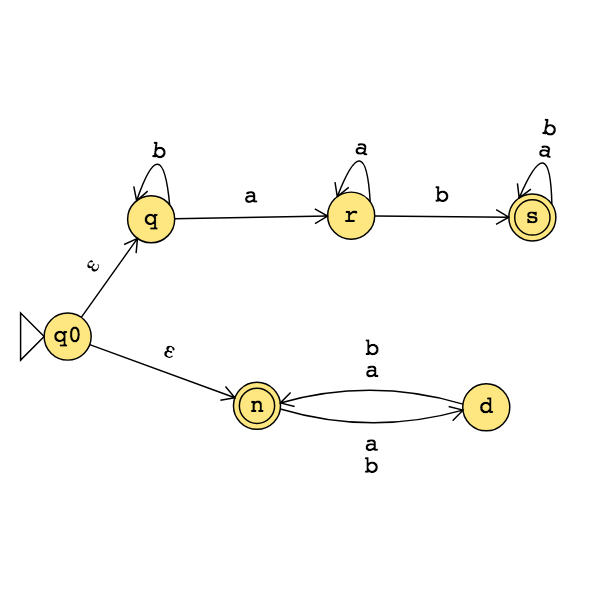
\includegraphics[width=2.5in]{../../resources/machines/Lect5NFA1.png}


\vspace{-10pt}

The language recognized by this NFA is: 